% !TeX spellcheck = en_US
\documentclass[11pt]{article}
\usepackage{amsmath}
\usepackage{steinmetz}
\usepackage{graphicx}
\usepackage{lipsum}
\usepackage[margin=2cm]{geometry}

%opening
\title{Configuraciones especiales y filtros activos}
\author{Juan Barbosa - 201325901}

\begin{document}

\maketitle

\section{Derivador}
Para una capacitancia, se define la impedancia como $Z_c = 1/j\omega c$. Teniendo en cuenta que existe realimentaci\'on negativa, la corriente por la capacitancia es la misma que pasa sobre la resistencia.
\begin{equation}
	\dfrac{V_{in}-V_N}{Z_c} = \dfrac{V_N-V_{out}}{R}
\end{equation}

\noindent como $V_N=V_P=0$
\begin{equation}
	V_{out}=-\dfrac{R}{Z_c}V_{in}=-j\omega RCV_{in}=-RC\dfrac{dV_{in}}{dt}
\end{equation}

\section{Integrador}
De forma an\'aloga, la corriente sobre la resistencia es la misma que atraviesa la capacitancia.
\begin{equation}
	\dfrac{V_{in}-V_N}{R} = \dfrac{V_N-V_{out}}{Z_c}
\end{equation}

\noindent dado que $V_N=V_P=0$
\begin{equation}
	V_{out}=-\dfrac{Z_c}{R}V_{in}=-\dfrac{1}{j\omega RC}V_{in}=-\dfrac{1}{RC}\int V_{in} dt
\end{equation}

\section{Filtro con amplificaci\'on}
Teniendo en cuenta que $C_1$ y $R_1$ est\'an en serie:
\begin{equation}
	Z_{eq} = Z_{c1} + R_1=\dfrac{1+j\omega R_1C}{j\omega C}
\end{equation}

\noindent A partir de los mismos argumentos anteriores,
\begin{equation*}
	\dfrac{V_{in}-V_N}{Z_{eq}}=\dfrac{V_N-V_{out}}{R_2}
\end{equation*}
\begin{equation}
	V_{out} = -\dfrac{R_2}{Z_{eq}}V_{in} = -\dfrac{j\omega R_2C}{1+j\omega R_1C} V_{in}
\end{equation}

\noindent Lo cual se puede escribir en notaci\'on fasorial como:
\begin{equation}
	V_{out} = \dfrac{C R_{2}\omega}{\sqrt{C^{2} R_{1}^{2} \omega^{2} + 1}} V_{in}\phase{\arctan\left(\dfrac{1}{R_1C\omega}\right)}
\end{equation}

\noindent La frecuencia de corte es entonces:
\begin{equation}
	\omega_c = \dfrac{1}{R_1C} \approx 1000 \text{ rad/s}
\end{equation}

\pagebreak
\begin{figure}[h]
	\centering
	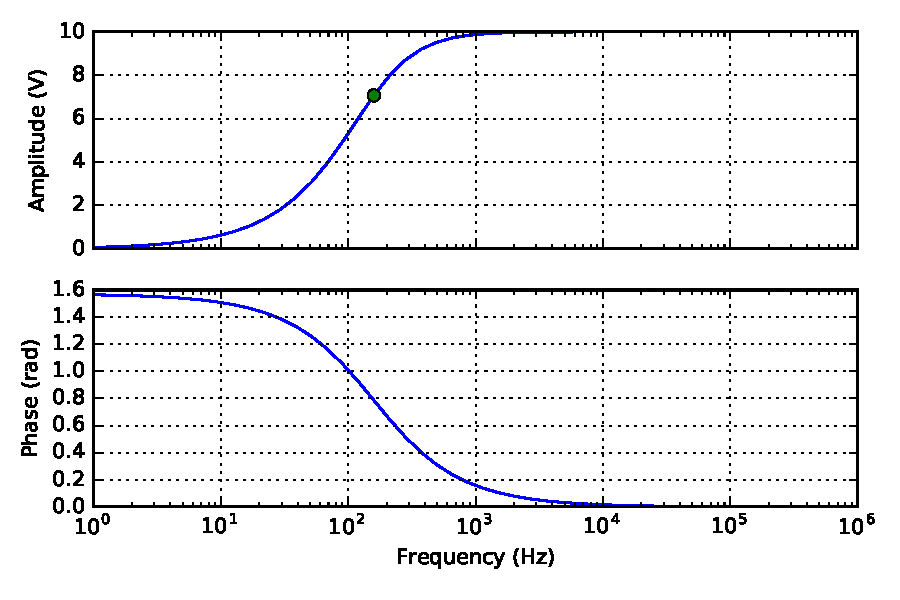
\includegraphics[width=0.5\linewidth]{filter.pdf}
	\caption{Amplitude and phase dependency with the frequency.}
\end{figure}

\section{Filtro pasabanda}
\end{document}
